\documentclass[aspectratio=169]{beamer}
\usetheme{Madrid}
\usepackage{booktabs}
\usepackage{graphicx}
\usepackage{siunitx}
\usepackage{pgfplots}
\usepackage{pgfplotstable}
\usepackage{hyperref}
\usepgfplotslibrary{statistics}
\pgfplotsset{compat=1.18,table/search path={data,../data}}
\pgfplotstableset{col sep=comma}
\sisetup{round-mode=places,round-precision=2}

% Resolve the CSV location regardless of where the slide deck is compiled.
\newif\ifredWineDataAvailable
\newcommand{\redWineDataPath}{}
\IfFileExists{data/red_wine_quality.csv}{%
  \redWineDataAvailabletrue
  \edef\redWineDataPath{\detokenize{data/red_wine_quality.csv}}%
}{%
  \IfFileExists{../data/red_wine_quality.csv}{%
    \redWineDataAvailabletrue
    \edef\redWineDataPath{\detokenize{../data/red_wine_quality.csv}}%
  }{%
    \redWineDataAvailablefalse
    \PackageWarningNoLine{video_presentation_slides}{Data file red\_wine\_quality.csv not found; data-driven plots will show placeholders.}%
  }%
}

\title{Exploratory Data Analysis of Red Wine Quality}
\subtitle{UCI Machine Learning Repository Dataset}
\author{Kevin Bell \\\ Angelie Reyes-Sosa \\\ Dani Lopez}
\date{Fall 2025}

\begin{document}

\begin{frame}
  \titlepage
\end{frame}

\begin{frame}{Agenda}
  \begin{itemize}
    \item Motivation and dataset overview
    \item Three guiding questions and hypotheses
    \item Evidence from descriptive statistics and visuals
    \item Key anomalies and synthesis of findings
    \item Future research plan and closing takeaways
  \end{itemize}
\end{frame}

\begin{frame}{Why This Dataset?}
  \begin{itemize}
    \item \textbf{Scope:} \num{1599} Portuguese \emph{Vinho Verde} red wines with \num{11} physicochemical features plus quality score.
    \item \textbf{Relevance:} Widely cited benchmark that still leaves room for actionable winemaking insights.
    \item \textbf{Course fit:} Easily satisfies requirements on feature count and observation size.
  \end{itemize}
\end{frame}

\begin{frame}{Feature Definitions}
  \scriptsize
  \begin{tabular}{p{0.32\textwidth}p{0.62\textwidth}}
    \toprule
    \textbf{Feature} & \textbf{Description} \\
    \midrule
    Fixed acidity & Non-volatile acids (g/dm\textsuperscript{3}). \\
    Volatile acidity & Acetic acid (g/dm\textsuperscript{3}); vinegar aromas. \\
    Citric acid & Adds freshness and structure (g/dm\textsuperscript{3}). \\
    Residual sugar & Sugar remaining post-fermentation (g/dm\textsuperscript{3}). \\
    Chlorides & Salt content (g/dm\textsuperscript{3}). \\
    Free sulfur dioxide & Protects against oxidation (mg/dm\textsuperscript{3}). \\
    Total sulfur dioxide & Combined bound and free SO\textsubscript{2} (mg/dm\textsuperscript{3}). \\
    Density & Proxy for sugar/alcohol balance (g/cm\textsuperscript{3}). \\
    pH & Acidity (unitless). \\
    Sulfates & Potassium sulfate (g/dm\textsuperscript{3}); antimicrobial. \\
    Alcohol & Ethanol percentage by volume. \\
    Quality & Median sensory rating (3--8 scale). \\
    \bottomrule
  \end{tabular}
\end{frame}

\begin{frame}{Guiding Questions \\ and Analytical Assumptions}
  \begin{enumerate}
    \item Which chemistry attributes best distinguish higher-quality wines?
    \item How do acidity profiles interact with sulfur management across quality tiers?
    \item Are there latent subgroups that signal distinct wine styles?
  \end{enumerate}
  \vspace{1em}
  \textbf{Assumptions and biases}
  \begin{itemize}
    \item Treat quality score as approximately continuous for correlation work.
    \item Lab measurements assumed unbiased; focus is chemistry-centric.
  \end{itemize}
\end{frame}

\begin{frame}{Working Hypotheses}
  \begin{itemize}
    \item Alcohol and sulfates will correlate positively with quality.
    \item Volatile acidity will correlate negatively with quality.
    \item Density and residual sugar play limited roles because most wines are dry.
  \end{itemize}
\end{frame}

\begin{frame}{Summary Statistics Highlights}
  \small
  \begin{tabular}{lS[table-format=2.2]S[table-format=1.2]S[table-format=1.2]S[table-format=1.2]S[table-format=1.3]S[table-format=1.2]}
    \toprule
    & {Alcohol} & {Vol. acidity} & {Citric acid} & {Sulfates} & {Density} & {pH} \\
    \midrule
    Mean & 10.42 & 0.53 & 0.27 & 0.66 & 0.997 & 3.31 \\
    Std. dev. & 1.07 & 0.18 & 0.20 & 0.17 & 0.002 & 0.15 \\
  \end{tabular}
  \vspace{0.75em}
  \begin{itemize}
    \item Alcohol and sulfates show the greatest relative spread \textrightarrow{} leverage for quality differentiation.
    \item Volatile acidity variability flags riskier sensory outcomes.
  \end{itemize}
\end{frame}

\begin{frame}{Means by Quality Tier}
  \scriptsize
  \begin{tabular}{cS[table-format=2.2]S[table-format=1.2]S[table-format=1.2]S[table-format=1.2]S[table-format=2.1]}
    \toprule
    \textbf{Quality} & {Alcohol} & {Vol. acidity} & {Citric acid} & {Sulfates} & {Total SO\textsubscript{2}} \\
    \midrule
    3 & 9.96 & 0.89 & 0.17 & 0.57 & 24.90 \\
    4 & 10.27 & 0.69 & 0.17 & 0.60 & 36.25 \\
    5 & 9.90 & 0.58 & 0.24 & 0.62 & 56.51 \\
    6 & 10.63 & 0.50 & 0.27 & 0.68 & 40.87 \\
    7 & 11.47 & 0.40 & 0.38 & 0.74 & 35.02 \\
    8 & 12.09 & 0.42 & 0.39 & 0.77 & 33.44 \\
    \bottomrule
  \end{tabular}
  \vspace{0.75em}
  \begin{itemize}
    \item Alcohol climbs steadily with quality while volatile acidity drops.
    \item Total SO\textsubscript{2} peaks at mid-tier quality, pointing to a sweet spot.
  \end{itemize}
\end{frame}

\begin{frame}{Alcohol vs. Quality}
  \ifredWineDataAvailable
    \begin{center}
      \begin{tikzpicture}
        \begin{axis}[
          width=0.9\textwidth,
          height=0.55\textheight,
          xlabel={Alcohol (\%)},
          ylabel={Quality score},
          ymin=2.5, ymax=8.5,
          grid=both,
          grid style={line width=.1pt, draw=gray!20},
          major grid style={line width=.2pt,draw=gray!50},
          scatter/classes={
            3={mark=*,draw=black,fill=red!60},
            4={mark=*,draw=black,fill=orange!70},
            5={mark=*,draw=black,fill=yellow!80!black},
            6={mark=*,draw=black,fill=green!70!black},
            7={mark=*,draw=black,fill=blue!70},
            8={mark=*,draw=black,fill=purple!70}
          },
          legend style={draw=none,at={(0.02,0.98)},anchor=north west,font=\scriptsize},
          legend cell align=left,
          scatter src=explicit symbolic
        ]
          \addplot+[only marks,opacity=0.35] table[
            x=alcohol,
            y=quality,
            meta=quality
          ] {\redWineDataPath};
          \addplot+[no marks,very thick,color=red!70!black,domain=8.4:14.9,forget plot]
            {0.360842 * x + 1.87497};
          \legend{3,4,5,6,7,8}
        \end{axis}
      \end{tikzpicture}
    \end{center}
    \vspace{-0.5em}
    \centering\small Positive slope reinforces alcohol as a top quality discriminator.
  \else
    \begin{center}
      \small Data file \texttt{red\_wine\_quality.csv} not found; plot omitted.
    \end{center}
  \fi
\end{frame}

\pgfplotstableread[col sep=space]{%
feature correlation
Alcohol 0.476
Sulfates 0.251
Citric_acid 0.226
Fixed_acidity 0.124
Residual_sugar 0.014
Free_sulfur_dioxide -0.051
pH -0.058
Chlorides -0.129
Density -0.175
Total_sulfur_dioxide -0.185
Volatile_acidity -0.391
}{\correlationtable}

\begin{frame}{Feature Correlations with Quality}
  \begin{tikzpicture}
    \begin{axis}[
      width=0.92\textwidth,
      height=0.55\textheight,
      ybar,
      bar width=8pt,
      symbolic x coords={Alcohol,Sulfates,Citric_acid,Fixed_acidity,Residual_sugar,Free_sulfur_dioxide,pH,Chlorides,Density,Total_sulfur_dioxide,Volatile_acidity},
      xtick=data,
      xticklabel style={rotate=60,anchor=east, font=\scriptsize},
      xticklabels={Alcohol,Sulfates,Citric acid,Fixed acidity,Residual sugar,Free SO\textsubscript{2},pH,Chlorides,Density,Total SO\textsubscript{2},Volatile acidity},
      ylabel={Correlation},
      ymin=-0.45,
      ymax=0.55,
      grid=both,
      grid style={line width=.1pt, draw=gray!15},
      major grid style={line width=.2pt, draw=gray!45}
    ]
      \addplot+ table[x=feature,y=correlation] {\correlationtable};
    \end{axis}
  \end{tikzpicture}
  \vspace{0.5em}
  \small Alcohol dominates; volatile acidity is the strongest negative signal.
\end{frame}

\begin{frame}{Volatile Acidity Tightens at Higher Quality}
  \begin{tikzpicture}
    \begin{axis}[
      width=0.92\textwidth,
      height=0.55\textheight,
      boxplot/draw direction=y,
      xtick={1,2,3,4,5,6},
      xticklabels={3,4,5,6,7,8},
      xlabel={Quality score},
      ylabel={Volatile acidity (g/dm\textsuperscript{3})},
      grid=both,
      grid style={line width=.1pt, draw=gray!20},
      major grid style={line width=.2pt,draw=gray!50}
    ]
      \addplot+[boxplot prepared={lower whisker=0.44,lower quartile=0.648,median=0.845,upper quartile=1.01,upper whisker=1.58}] coordinates {};
      \addplot+[boxplot prepared={lower whisker=0.23,lower quartile=0.53,median=0.67,upper quartile=0.87,upper whisker=1.13}] coordinates {};
      \addplot+[boxplot prepared={lower whisker=0.18,lower quartile=0.46,median=0.58,upper quartile=0.67,upper whisker=1.33}] coordinates {};
      \addplot+[boxplot prepared={lower whisker=0.16,lower quartile=0.38,median=0.49,upper quartile=0.60,upper whisker=1.04}] coordinates {};
      \addplot+[boxplot prepared={lower whisker=0.12,lower quartile=0.30,median=0.37,upper quartile=0.485,upper whisker=0.915}] coordinates {};
      \addplot+[boxplot prepared={lower whisker=0.26,lower quartile=0.335,median=0.37,upper quartile=0.473,upper whisker=0.85}] coordinates {};
    \end{axis}
  \end{tikzpicture}
  \vspace{0.5em}
  \small Higher scores cluster at lower, tighter volatility levels.
\end{frame}

\begin{frame}{Acidity and Sulfur Dioxide Interplay}
  \ifredWineDataAvailable
    \begin{center}
      \begin{tikzpicture}
        \begin{axis}[
          width=0.9\textwidth,
          height=0.55\textheight,
          xlabel={Volatile acidity (g/dm\textsuperscript{3})},
          ylabel={Total SO\textsubscript{2} (mg/dm\textsuperscript{3})},
          xmin=0, xmax=1.5,
          ymin=-20, ymax=170,
          grid=both,
          grid style={line width=.1pt, draw=gray!20},
          major grid style={line width=.2pt,draw=gray!50},
          scatter/classes={
            3={mark=*,draw=black,fill=red!60},
            4={mark=*,draw=black,fill=orange!70},
            5={mark=*,draw=black,fill=yellow!80!black},
            6={mark=*,draw=black,fill=green!70!black},
            7={mark=*,draw=black,fill=blue!70},
            8={mark=*,draw=black,fill=purple!70}
          },
          legend style={draw=none,at={(0.02,0.98)},anchor=north west,font=\scriptsize},
          legend cell align=left,
          scatter src=explicit symbolic
        ]
          \addplot+[only marks,opacity=0.35] table[
            x=volatile_acidity,
            y=total_sulfur_dioxide,
            meta=quality
          ] {\redWineDataPath};
          \legend{3,4,5,6,7,8}
        \end{axis}
      \end{tikzpicture}
    \end{center}
    \vspace{-0.4em}
    \centering\small High volatility with heavy sulfur shows up mostly in lower-quality wines.
  \else
    \begin{center}
      \small Data file \texttt{red\_wine\_quality.csv} not found; plot omitted.
    \end{center}
  \fi
\end{frame}

\begin{frame}{Interaction Model Insights}
  \small
  \begin{tabular}{lS[table-format=1.3]}
    \toprule
    Term & {Coefficient} \\
    \midrule
    Intercept & 5.684 \\
    Volatile acidity & -1.033 \\
    Sulphates & 1.198 \\
    Volatile acidity $\times$ sulphates & -0.858 \\
    \bottomrule
  \end{tabular}
  \vspace{1em}
  \begin{itemize}
    \item Model: $R^2 = 0.177$ on quality using volatility, sulphates, and their interaction.
    \item Negative interaction \textrightarrow{} sulphates help most when volatility is already controlled.
  \end{itemize}
\end{frame}

\begin{frame}{Sulfur Response by Quality Tier}
  \scriptsize
  \begin{tabular}{cS[table-format=3.2]S[table-format=1.3]S[table-format=1.3]}
    \toprule
    \textbf{Quality} & {Slope (mg/dm\textsuperscript{3} per g/dm\textsuperscript{3})} & {Correlation} & {Mean sulphates} \\
    \midrule
    3 & -27.39 & -0.539 & 0.570 \\
    4 & -17.04 & -0.136 & 0.596 \\
    5 & 1.97 & 0.009 & 0.621 \\
    6 & 7.37 & 0.047 & 0.675 \\
    7 & 4.69 & 0.021 & 0.741 \\
    8 & 76.26 & 0.434 & 0.768 \\
    \bottomrule
  \end{tabular}
  \vspace{0.75em}
  \begin{itemize}
    \item Low-quality wines: sulfur dioxide drops as volatility rises.
    \item Elite wines: positive slope suggests balanced sulphur supports stability without sensory penalties.
  \end{itemize}
\end{frame}

\pgfmathsetmacro{\meanfixed}{8.319637}
\pgfmathsetmacro{\stdfixed}{1.740552}
\pgfmathsetmacro{\pcafixedone}{-0.489314}
\pgfmathsetmacro{\pcafixedtwo}{-0.110503}
\pgfmathsetmacro{\meanvolatile}{0.527821}
\pgfmathsetmacro{\stdvolatile}{0.179004}
\pgfmathsetmacro{\pcavolone}{0.238584}
\pgfmathsetmacro{\pcavoltwo}{0.274930}
\pgfmathsetmacro{\meancitric}{0.270976}
\pgfmathsetmacro{\stdcitric}{0.194740}
\pgfmathsetmacro{\pcacitone}{-0.463632}
\pgfmathsetmacro{\pcacittwo}{-0.151791}
\pgfmathsetmacro{\meanresidual}{2.538806}
\pgfmathsetmacro{\stdresidual}{1.409487}
\pgfmathsetmacro{\pcaresone}{-0.146107}
\pgfmathsetmacro{\pcaRestwo}{0.272080}
\pgfmathsetmacro{\meanchlorides}{0.087467}
\pgfmathsetmacro{\stdchlorides}{0.047051}
\pgfmathsetmacro{\pcachlorone}{-0.212247}
\pgfmathsetmacro{\pcachlortwo}{0.148052}
\pgfmathsetmacro{\meanfree}{15.874922}
\pgfmathsetmacro{\stdfree}{10.456886}
\pgfmathsetmacro{\pcafreeone}{0.036158}
\pgfmathsetmacro{\pcafreetwo}{0.513567}
\pgfmathsetmacro{\meantotal}{46.467792}
\pgfmathsetmacro{\stdtotal}{32.885037}
\pgfmathsetmacro{\pcatotalone}{-0.023575}
\pgfmathsetmacro{\pcatotaltwo}{0.569487}
\pgfmathsetmacro{\meandensity}{0.996747}
\pgfmathsetmacro{\stddensity}{0.001887}
\pgfmathsetmacro{\pcadensityone}{-0.395353}
\pgfmathsetmacro{\pcadensitytwo}{0.233575}
\pgfmathsetmacro{\meanph}{3.311113}
\pgfmathsetmacro{\stdph}{0.154338}
\pgfmathsetmacro{\pcaphone}{0.438520}
\pgfmathsetmacro{\pcaphtwo}{0.006711}
\pgfmathsetmacro{\meansulphates}{0.658149}
\pgfmathsetmacro{\stdsulphates}{0.169454}
\pgfmathsetmacro{\pcasulphone}{-0.242921}
\pgfmathsetmacro{\pcasulptwo}{-0.037554}
\pgfmathsetmacro{\meanalcohol}{10.422983}
\pgfmathsetmacro{\stdalcohol}{1.065334}
\pgfmathsetmacro{\pcaalcoholone}{0.113232}
\pgfmathsetmacro{\pcaalcoholtwo}{-0.386181}

\ifredWineDataAvailable
  \pgfplotstableread{\redWineDataPath}{\pcatable}
  \pgfplotstablecreatecol[
    create col/expr={
      ((\thisrow{fixed_acidity}-\meanfixed)/\stdfixed)*\pcafixedone +
      ((\thisrow{volatile_acidity}-\meanvolatile)/\stdvolatile)*\pcavolone +
      ((\thisrow{citric_acid}-\meancitric)/\stdcitric)*\pcacitone +
      ((\thisrow{residual_sugar}-\meanresidual)/\stdresidual)*\pcaresone +
      ((\thisrow{chlorides}-\meanchlorides)/\stdchlorides)*\pcachlorone +
      ((\thisrow{free_sulfur_dioxide}-\meanfree)/\stdfree)*\pcafreeone +
      ((\thisrow{total_sulfur_dioxide}-\meantotal)/\stdtotal)*\pcatotalone +
      ((\thisrow{density}-\meandensity)/\stddensity)*\pcadensityone +
      ((\thisrow{ph}-\meanph)/\stdph)*\pcaphone +
      ((\thisrow{sulphates}-\meansulphates)/\stdsulphates)*\pcasulphone +
      ((\thisrow{alcohol}-\meanalcohol)/\stdalcohol)*\pcaalcoholone
    }
  ]{pcone}{\pcatable}
  \pgfplotstablecreatecol[
    create col/expr={
      ((\thisrow{fixed_acidity}-\meanfixed)/\stdfixed)*\pcafixedtwo +
      ((\thisrow{volatile_acidity}-\meanvolatile)/\stdvolatile)*\pcavoltwo +
      ((\thisrow{citric_acid}-\meancitric)/\stdcitric)*\pcacittwo +
      ((\thisrow{residual_sugar}-\meanresidual)/\stdresidual)*\pcaRestwo +
      ((\thisrow{chlorides}-\meanchlorides)/\stdchlorides)*\pcachlortwo +
      ((\thisrow{free_sulfur_dioxide}-\meanfree)/\stdfree)*\pcafreetwo +
      ((\thisrow{total_sulfur_dioxide}-\meantotal)/\stdtotal)*\pcatotaltwo +
      ((\thisrow{density}-\meandensity)/\stddensity)*\pcadensitytwo +
      ((\thisrow{ph}-\meanph)/\stdph)*\pcaphtwo +
      ((\thisrow{sulphates}-\meansulphates)/\stdsulphates)*\pcasulptwo +
      ((\thisrow{alcohol}-\meanalcohol)/\stdalcohol)*\pcaalcoholtwo
    }
  ]{pctwo}{\pcatable}
\fi

\begin{frame}{Principal Components Overview}
  \begin{columns}[T,totalwidth=\textwidth]
    \begin{column}{0.45\textwidth}
      \small
      \begin{tabular}{lS[table-format=1.3]}
        \toprule
        Component & {Variance explained} \\
        \midrule
        PC1 & 0.282 \\
        PC2 & 0.175 \\
        PC3 & 0.141 \\
        \bottomrule
      \end{tabular}
    \end{column}
    \begin{column}{0.5\textwidth}
      \scriptsize
      \begin{tabular}{lS[table-format=1.3]S[table-format=1.3]}
        \toprule
        Feature & {PC1} & {PC2} \\
        \midrule
        Fixed acidity & -0.489 & -0.111 \\
        Citric acid & -0.464 & -0.152 \\
        Density & -0.395 & 0.234 \\
        pH & 0.439 & 0.007 \\
        Volatile acidity & 0.239 & 0.275 \\
        Free SO\textsubscript{2} & 0.036 & 0.514 \\
        Total SO\textsubscript{2} & -0.024 & 0.569 \\
        Residual sugar & -0.146 & 0.272 \\
        Alcohol & 0.113 & -0.386 \\
        \bottomrule
      \end{tabular}
    \end{column}
  \end{columns}
  \vspace{0.5em}
  \small PC1 balances structural acidity against pH/alcohol; PC2 captures sulphur management and sweetness.
\end{frame}

\begin{frame}{PCA Projection by Quality}
  \ifredWineDataAvailable
    \begin{center}
      \begin{tikzpicture}
        \begin{axis}[
          width=0.9\textwidth,
          height=0.55\textheight,
          xlabel={PC1 score},
          ylabel={PC2 score},
          grid=both,
          grid style={line width=.1pt, draw=gray!20},
          major grid style={line width=.2pt,draw=gray!50},
          scatter/classes={
            3={mark=*,draw=black,fill=red!60},
            4={mark=*,draw=black,fill=orange!70},
            5={mark=*,draw=black,fill=yellow!80!black},
            6={mark=*,draw=black,fill=green!70!black},
            7={mark=*,draw=black,fill=blue!70},
            8={mark=*,draw=black,fill=purple!70}
          },
          legend style={draw=none,at={(0.02,0.98)},anchor=north west,font=\scriptsize},
          legend cell align=left,
          scatter src=explicit symbolic
        ]
          \addplot+[only marks,opacity=0.35] table[
            x=pcone,
            y=pctwo,
            meta=quality
          ] {\pcatable};
          \legend{3,4,5,6,7,8}
        \end{axis}
      \end{tikzpicture}
    \end{center}
    \vspace{-0.4em}
    \centering\small Quality 7--8 wines cluster with positive PC1 and moderate PC2 scores.
  \else
    \begin{center}
      \small Data file \texttt{red\_wine\_quality.csv} not found; PCA projection omitted.
    \end{center}
  \fi
\end{frame}

\begin{frame}{K-means Segmentation}
  \small
  \begin{columns}[T,totalwidth=\textwidth]
    \begin{column}{0.48\textwidth}
      \centering
      \scriptsize
      \begin{tabular}{cS[table-format=1.3]S[table-format=5.2]}
        \toprule
        $k$ & {Silhouette} & {Inertia} \\
        \midrule
        2 & 0.207 & 14330.94 \\
        3 & 0.172 & 12884.10 \\
        4 & 0.145 & 12044.58 \\
        5 & 0.166 & 10828.29 \\
        \bottomrule
      \end{tabular}
      \vspace{0.4em}
      \scriptsize Best silhouette achieved with two clusters.
    \end{column}
    \begin{column}{0.48\textwidth}
      \centering
      \scriptsize
      \begin{tabular}{lS[table-format=4.0]S[table-format=1.2]S[table-format=2.2]S[table-format=1.3]S[table-format=1.3]}
        \toprule
        Cluster & {Size} & {Mean quality} & {Alcohol} & {Vol. acidity} & {Sulfates} \\
        \midrule
        1 & 638 & 5.870 & 10.578 & 0.418 & 0.745 \\
        0 & 961 & 5.481 & 10.320 & 0.601 & 0.600 \\
        \bottomrule
      \end{tabular}
      \vspace{0.4em}
      \scriptsize Cluster 1 = premium chemistry; Cluster 0 = mainstream baseline.
    \end{column}
  \end{columns}
  \vspace{0.4em}
  \small Segmentation aligns with the PCA structure and highlights actionable chemistry targets.
\end{frame}

\begin{frame}{Notable Anomalies}
  \begin{itemize}
    \item Sulfate-heavy outliers: extreme additions with high volatility remain stuck in quality 3--4 despite sulphate boosts.
    \item High-chloride, low-quality samples merit lab re-checks and potential process audits.
  \end{itemize}
\end{frame}

\begin{frame}{Synthesis}
  \begin{itemize}
    \item High-scoring wines: higher alcohol, moderate sulfates, elevated citric acid, lower volatile acidity.
    \item Interaction model: sulphates help only when volatility is controlled, matching the acidity--sulfur scatter.
    \item PCA and k-means: 961-wine mainstream cluster vs. 638-wine premium segment with disciplined sulphate management.
  \end{itemize}
\end{frame}

\begin{frame}{Future Research and Predictive Plan}
  \begin{enumerate}
    \item Build predictive models (regularized regression, gradient boosting, tree ensembles) with key interactions.
    \item Explore segmentation beyond two clusters using Gaussian mixtures or density-based methods, validating with silhouette and stability diagnostics.
    \item Simulate chemistry adjustments with causal inference tools (e.g., propensity score weighting).
  \end{enumerate}
  \vspace{0.5em}
  \small Additional questions: missing vintage/producer effects? blending strategies to mitigate deficiencies?
\end{frame}

\begin{frame}{Conclusion}
  \begin{itemize}
    \item Met objectives: characterized data, answered core questions, charted next steps.
    \item Key takeaways: alcohol and balanced sulfates aid quality; volatile acidity detracts; actionable subgroups emerge.
    \item Thank you! Report and repository contain full reproducible analysis.
  \end{itemize}
\end{frame}

\begin{frame}[standout]
  Questions?\newline
  \small Team: Kevin Bell, Angelie Reyes-Sosa, Dani Lopez\
\end{frame}

\end{document}
